\section{Présentation générale}

\subsection{Schémas}

Concernant l’intégration des différents blocs avec les blocs existant, celle-ci doit être faite en respectant des standards qui permettront à terme de maximiser les performances de l’architecture applicative en terme de capacités d’intégration de nouveaux blocs. Cette capacité d’intégration repose sur l’utilisation d’un standard et donc une normalisation des échanges et des flux de données entre les différentes applications. \\

Nous proposons donc de baser notre intégration sur le modèle proposé par DataXtend Semantic Integrator (DXSI). Cette solution permet, en effet, de standardiser les échanges et de faciliter la maintenance des blocs existant et l’intégration de nouveaux blocs. Cette solution est également accessible car elle propose des outils pour éditer directement les modèles de données manipulés par la pile logiciel d’intégration. \\

Cette solution nécessitera néanmoins un travail d’ampleur pour développer les adaptateurs nécessaires pour intégrer les outils existant. Les figures suivantes montrent l’objectif à atteindre à l’issue de la phase de développement. \\
    
La phase de  développement devra commencer par la concevoir le modèle de données commun (Common Data Model) et de mettre en place le bus. Une fois cette première étape terminée, la suivante consistera à développer les adaptateurs pour les applications existantes. Chaque adaptateur pourra être développer en parallèle car il est spécifique au bloc le concernant. L’ultime étape de développement pourra être la réalisation des nouveaux blocs et de leurs interfaces avec le bus. Ces deux dernières phases pourront être réalisées en parallèle, chaque tâche les constituant pouvant elle même être parallélisée. \\

\begin{figure}[H]
    \label{fig-bus}
    \noindent\makebox[\textwidth]{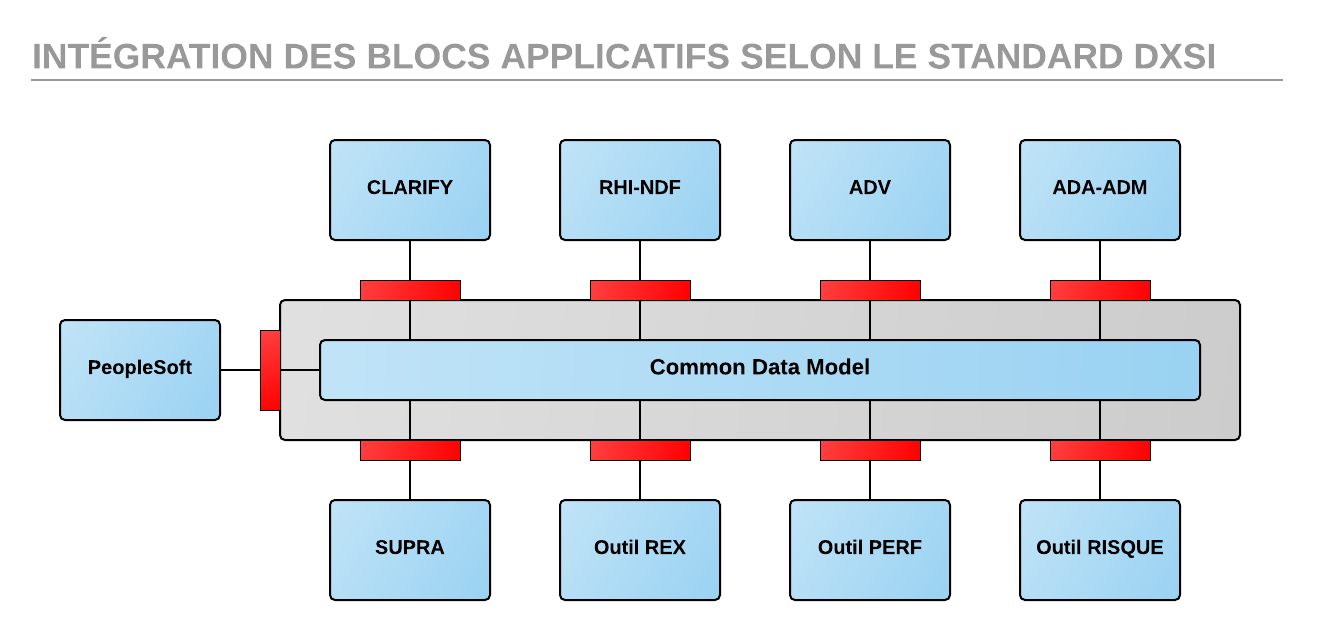
\includegraphics[width=12cm]{figures/schema_integration.png}}
    \caption{Schéma de la structure d'intégration théorique}
\end{figure}

\subsection{Problématiques}

De nombreux problèmes peuvent se poser lors de la mise en place d’une nouvelle application dans une architecture existante. En effet, faire communiquer différentes applications demande un développement d’adaptateur qui n’est pas toujours aisé et cela nécessite du temps. 

Il est également envisageable de rencontrer des problèmes de synchronisation entre les applications. Il est impossible d’effectuer une opération sur des données n’étant pas encore prises en compte dans le système.

Enfin il est important de noter que le changement de comportement d’une application peut potentiellement entraîner des changements aux niveau de l’adaptateur associé.

\section{Intégration \& architecture technique}

\subsection{Solutions pour l’intégration des nouveaux blocs}

Afin d’intégrer les différentes solutions permettant de répondre aux problèmes soulevés par les trois axes nous allons mettre en place un middleware d’intégration entre le logiciel PeopleSoft et les nouvelles solutions qui seront mises en place. Cela aura deux avantages majeurs, le premier étant la garantie de l’évolutivité du système mis en place et le second la normalisation des échanges entre les nouveaux composants. Le schéma suivant présente les différents composants à mettre en place.

\begin{figure}[H]
    \label{fig-bus-theo}
    \noindent\makebox[\textwidth]{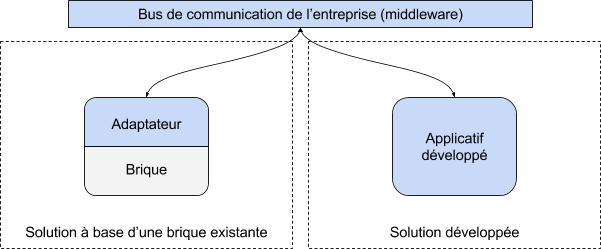
\includegraphics[width=12cm]{figures/schema_integration_theorique.png}}
    \caption{Schéma de la structure d'intégration théorique}
\end{figure}

On constate sur ce schéma différents éléments qu’il sera nécessaire de développer. Il faudra développer l’intégralité des composants de type “Adaptateur” pour chaque solution à base de brique existante et pour l’existant c’est-à-dire l’ensemble PeopleSoft et les applicatifs qui gravitent autour. Lors de la réalisation d’une solution intégralement développée il sera nécessaire que celle-ci intègre directement le protocole de communication sur le bus afin de ne pas ajouter le développement d’un adaptateur. \\
    
Il est évidemment nécessaire de définir un format d’échange des données pour une architecture de ce type. Les format de données semi-structurées de type XML, JSON sont sans doute les plus répandus et les plus adaptés pour ce type d’architecture. \\

Le bus n’est destiné qu’à la transmission des messages et ne doit effectuer aucun traitement sur ces derniers. Il doit juste orienté les messages reçu vers les applications destinataires de ces messages. \\

Le rôle des adaptateurs est d’effectuer les opérations de traduction réciproques permettant de passer d’un message de l’application à un message pouvant circuler sur le bus. \\

Il faut cependant faire attention au format et au nombre de données envoyées sur le bus. Il peut être difficile de définir un format de message suffisamment riche pour permettre à toutes les applications de communiquer de manière efficace avec l’intégralité des informations qu’elle souhaite diffuser. \\

Afin d’éviter un problème de synchronisation, la communication sur bus nécessite de définir quelques règles concernant l’asynchronisme et l’ordre des messages. 

\subsection{Avantages de la solution spécifique}

La mise en place de cette solution spécifique apporte de nombreux avantages. Tout d’abord, les applications pourront être développées sur mesure et pourront ainsi parfaitement correspondre aux attentes et besoins de SPIE Sud-Est, augmentant de fait leur qualité de prestation. L’interface pourra également être définie selon les besoins et les fonctionnalités, personnalisant selon les habitudes des employés de SPIE Sud-Est les interactions avec les nouvelles applications mises à disposition. \\

Dans la même optique de mise en confort des utilisateurs, l’usage des nouveaux outils n’imposera pas forcément l’introduction ou la modification d’un processus existant, les nouvelles applications s’adaptant à ces derniers. Les utilisateurs n’auront donc pas à changer l’intégralité de leurs méthodes de travail. \\

Comme présenté précédemment, la nouvelle architecture applicative dispose d’une modularité grandement supérieure à l’ancienne organisation du système d’information de SPIE Sud-Est. En effet, la mise en place d’une solution de middleware d’intégration, basée sur un modèle de données commun, permettra par la suite d’ajouter facilement de nouvelles applications et fonctionnalités. \\

Enfin, cette solution permet une maîtrise totale de l’architecture applicative et de l’indépendance vis à vis des orientations prises par le développement d’un outil tiers. \\
